\providecommand{\main}{../..}
\documentclass[\main/main.tex]{subfiles}
\begin{document}

\chapter{Algoritmi probabilistici}
Gli algoritmi probabilistici richiedono un numero minore di calcoli degli algoritmi deterministici e quindi determinano una soluzione in un tempo minore. Esistono principalmente due famiglie di algoritmi probabilistici:

\begin{enumerate}
	\item Per cercare una soluzione esatta.
	\item Per cercare una soluzione approssimata.
\end{enumerate}

Per \textbf{algoritmi Monte-Carlo} si intendono gli algoritmi della categoria \textbf{1-sided error} e \textbf{2-sided error}.

Generalmente, per diminuire la probabilità di errore viene reiterato l'algoritmo probabilistico per un numero di volte ottenuto utilizzando la \textbf{disequazione di Chernoff} sino a che l'errore è inferiore ad un \(\delta \) accettabile.

\begin{figure}
	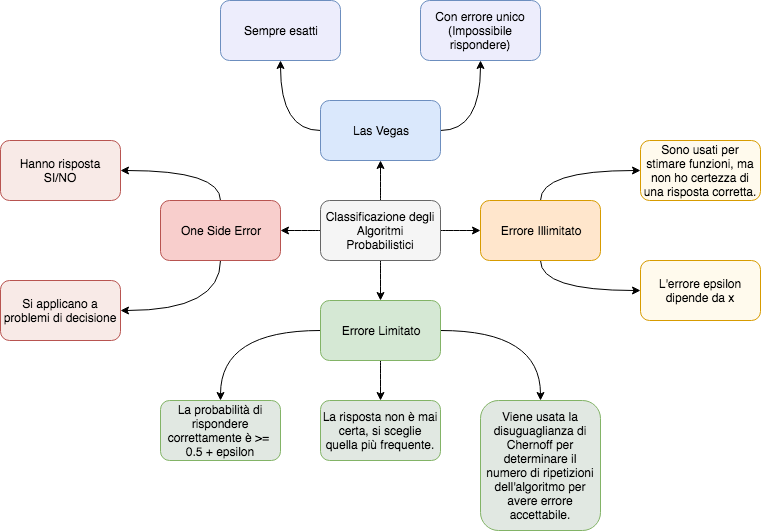
\includegraphics[width=\textwidth]{Mappa_algoritmi_probabilistici.png}
	\caption{Mappa degli algoritmi probabilistici}
\end{figure}

\section{1-Sided Error}
Hanno risposta SI/NO e vengono applicati a problemi di decisione.

\subsection{Esempio: Problema di protocollo di comunicazione}
Si vuole determinare se due stringhe binarie \(a\) e \(b\), lunghe \(n\), salvate su due terminali separati sono uguali senza inviare una stringa completamente da un terminale all'altro.

Un approccio banale risolverebbe in \(n\) messaggi il problema.

Un approccio sofisticato utilizza i resti della divisione con numeri primi. Dato un numero primo \(p \in \crl{2, \ldots, n^2}\) con probabilità uniforme, di dimensione \(\ceil{2\log_2{n}}\) bit.

\[
	r_a = \text{resto}\rnd{\frac{a}{p}} \in \crl{0,1, \ldots, p-1} \qquad r_b = \text{resto}\rnd{\frac{b}{p}} \in \crl{0,1, \ldots, p-1}
\]

\[
	r_a \neq r_b \Rightarrow a \neq b
\]

\[
	r_a = r_b \Rightarrow a \text{ potrebbe essere uguale a } b
\]

I valori del resto e di \(p\) sono inviati al secondo dei due nodi usando al più \(2\ceil{2\log_2{n}}\) bit, dove viene ripetuta la divisione ed effettuato il controllo, rispondendo con un bit se diversi o zero se uguali.

Se \(\mathcal{A}\) restituisce ``diverso'' la risposta è certamente corretta, mentre se restituisce ``uguale'' potrebbe essere sbagliato, con una probabilità pari a:

\[
	\prob{\text{errore}}{\mathcal{A}\text{ dice uguali}} = \prob{p \text{ divide }a-b}{a \neq b}
\]

Usando il \textbf{teorema dei numeri primi} che enuncia:

\begin{theorem}[Teorema dei numeri primi]
	Se \(\text{prim}(m) = \#\crl{i \in \crl{2, \ldots, m}: i \text{ è primo}}\) allora vale che:

	\[
		\text{prim}(m) \approx \frac{m}{\ln m} \qquad \text{ ovvero } \qquad \frac{\text{prim}(m)}{m}\ln m \longrightarrow 1
	\]

	Inoltre è noto che:

	\[
		\forall m > 67, \text{prim}(m) > \frac{m}{\ln m}
	\]
	Ogni numero intero di \(k\) bit possiede al più \(k-1\) divisori primi.
\end{theorem}

Si determina che la probabilità di scegliere un certo \(p\) risulta essere pari a:

\[
	\prob{p} = \frac{1}{\text{prim}\rnd{n^2}}, \qquad \prob{\text{errore}} = \frac{\arity{i \in \crl{1, \ldots, n^2}, i \text{ primo e divisore di }a-b}}{\text{prim}\rnd{n}^2}
\]

\[
	\prob{\text{errore}} \leq \frac{n-1}{\sfrac{n^2}{2\log_2 n}} \leq \frac{2\log_2 n}{n} \longrightarrow 0
\]

\[
	\prob{\text{errore}} \leq 10^{-14}
\]

Anche per \(n\) piccolo, se \(\frac{2\ln n}{n} < \frac{1}{2}\) ripeto l'algoritmo \(t\) volte ed ottengo una probabilità di errore pari a \(\prob{\text{errore}} < \frac{1}{2}^t\)

\subsection{Esempio: commutatività di matrici}
L'approccio deterministico usualmente termina in \(\O{k^3}\) o \(\O{k^\alpha}\) con \(2 < \alpha < 3\).

La procedura probabilistica cerca di determinare se \(\matr{A}\matr{B} \neq \matr{B}\matr{A}\).


\IncMargin{1em}
\begin{algorithm}
	\SetKwInOut{Input}{input}
	\SetKwInOut{Output}{output}
	\Input{\(\matr{A} = \rnd{A[1], \ldots, A[n]}, A \in \mathbb{U}^n\)}
	\Output{Il \(k\)-esimo elemento di \(A\)}
	\BlankLine
	\Begin{
		Scegli \(\bm{a} \in \crl{-1, 1}^k\) a caso in modo uniforme\;

		\(\bmu = \rnd{\bm{a}'\cdot \matr{A}}\matr{B}\)\;
		\(\bmv = \rnd{\bm{a}'\cdot \matr{B}}\matr{A}\)\;

		\If{\(\bmu \neq \bmv\)}{
			\Return ``Sono diverse''\;
		}
		\Else{
			\Return ``Sono uguali''\;
		}
	}
	\caption{Commutatività di matrici}
\end{algorithm}\DecMargin{1em}

\[\prob{\text{errore}} = \prob{\bmu=\bmb, \matr{A}\matr{B} = \matr{B}\matr{A}}\]

\[
	\matr{C} = \matr{A}\matr{B} - \matr{B}\matr{A} \neq 0 \Rightarrow \exists \text{ una colonna di } \matr{C}: \bmc_i \neq \bm{0}
\]

Supponiamo che \(\bmc_i \neq \bm{0}\), sapendo che \(\bm{a}\matr{A}\matr{B} = \bm{a}\matr{B}\matr{A}\). Prendiamo \(\bm{a} = \begin{bmatrix}
	a_1 & a_2 & \ldots & a_k
\end{bmatrix}, a_i \in \crl{-1, 1}\). Il prodotto quando \(\bmu = \bmv \) risulta essere:

\[
	\bm{a}'\matr{A}\matr{B} = \bm{a}'\matr{B}\matr{A} \Rightarrow \bm{a}'\bmc = 0 \Rightarrow \bm{a}' \begin{bmatrix}
		c_1    \\
		\vdots \\
		c_k
	\end{bmatrix} = 0 \Rightarrow \sum_{i=1}^k a_i c_i = 0
\]

Modifichiamo il vettore:
\[
	\bma = \begin{bmatrix}
		-1 & a_2 & \ldots & a_k
	\end{bmatrix}
	\qquad
	\bm{\beta} = \begin{bmatrix}
		1 & a_2 & \ldots & a_k
	\end{bmatrix}
\]
Uno di questi due vettori deve coincidere con \(A\).

\[
	\bma' \matr{C} \quad \lor \quad \bm{\beta}'\matr{C} = 0
\]

È importante notare che non può capire che entrambe le relazioni siano vere allo stesso tempo poiché implicherebbe, ricordando la premessa \(\bmc_i \neq 0\), che \(\bmc_i = 0\).

\section{Las Vegas}
Sono sempre esatti o ritornano `impossibile determinare soluzione' (spesso rappresentato con un punto di domanda).

\subsection{Esempio: RSEL}
Si tratta di un algoritmo \textbf{Las Vegas} utilizzato per estrarre il \(k\)-esimo elemento da un vettore definito su dominio \(\mathbb{U}\) totalmente ordinato (non esistono termini intercambiabili nell'ordine).

\IncMargin{1em}
\begin{algorithm}
	\SetKwInOut{Input}{input}
	\SetKwInOut{Output}{output}
	\Input{\(A, B \in \N^{k\times k}\)}
	\Output{Il \(k\)-esimo elemento di \(A\)}
	\BlankLine
	\Begin{
		\If{n=2}{
			Risolvi il problema direttamente.
		}
		\Else{
			Scegli \(t \in \crl{1, 2, \ldots, n}\) a caso in modo uniforme.\;
			Calcola \(A \leq \crl{A[j], A[j] < A[t]}\).\;
			Calcola \(A \geq \crl{A[j], j \neq t, A[j] \geq A[t]}\).\;

			\uIf{\(\arity{A} \leq k-1\)}{
				\Return \(A[t]\)
			}
			\uElseIf{\(\arity{A_<} \geq k\)}{
				\Return \(\text{RSEL}\rnd{A_<, k}\)
			}
			\Else{
				\Return \(\text{RSEL}\rnd{A_>, k- \arity{A_<} -1}\)
			}
		}
	}
	\caption{RSEL}
\end{algorithm}\DecMargin{1em}

\[
	T(n,k) \leq T_{\text{Quicksort}}(n)
\]
\begin{description}
	\item[Caso pessimo] \(T(n,k) = \O{n^2}\)
	\item[Caso medio] \(T(n,k) = \O{n\log{n}}\)
\end{description}

\subsection{Esempio: Quicksort}
Dato \(\mean{n}\), numero medio di confronti richiesto da \textbf{Quicksort} su un input di \(n\) elementi determinato come:

\[
	\mean{n} = (n+1) + \frac{1}{n}\sum_{k=0}^{n-1} \sqr{\mean{k} + \mean{n-1-k}}
\]
Usando il corollario del \textbf{teorema delle probabilità totali} che ricordiamo essere:

\formulaProbTot{}

Ottengo che i \textbf{tempo di calcolo che Quicksort} impiegati con un input di dimensione \(n\) sono pari a:

\[
	\mean{T_n} = \sum_{i = 0}^{n-1} \mean{T_n}{B_i} \prob{B_i} = n-1 + \sum_{i = 0}^{n-1} \mean{T_i} + \mean{T_{n-1-i}}
\]
\[
	\mean{n} = 2(n+1)H_n - 4n
\]

Dove \(H_n\) è l'\(n\)-esimo numero armonico, cioè \(H_n = \sum_{i=1}^n \frac{1}{i}\).

\subsection{Numero medio di confronti in RSEL}
\[
	T(n,k) = n-1 + \frac{1}{n}\sum_{l=k}^{n-1} T(l,k) + \frac{1}{n} \frac{1}{n}\sum_{l=0}^{k-2} T(n-1-l, k-l-1)
\]
Con \(k\leq n, \arity{A_<} = l\).

\subsection{Esempio: Protocollo 10}
Si tratta di un algoritmo \textbf{Las Vegas} per la comunicazione, che vuole stabilire se esiste un termine condiviso tra le due liste: \(\exists i: x_i = y_i\).

\begin{align*}
	A & : x_i, x_2, \ldots, x_10, \qquad x_i \in \crl{0,1}^n \qquad \forall i \in 1, \ldots, 10 \\
	B & : y_i, y_2, \ldots, y_10, \qquad y_i \in \crl{0,1}^n \qquad \forall i \in 1, \ldots, 10
\end{align*}

\begin{enumerate}
	\item \(A\) genera 10 numeri primi \(p_1, p_2, \ldots, p_10\), anche uguali, poiché estratti a caso in modo uniforme in \(\sqr{0, n^2}\).
	      \subitem \(A\) calcola \(r_i = \text{resto}\rnd{\frac{x_i}{p_i}} \quad \forall i, \ldots, 10\)
	      \subitem \(A\) invia le 10 coppie di resti e numeri primi.
	\item \(B\) calcola \(s_i = \text{resto}\rnd{\frac{y_i}{p_i}} \quad i = 1, \ldots, 10\).
	      \subitem Se sono tutti diversi allora \(B\) risponde ``NO''.
	      \subitem Altrimenti sia \(j=\min\crl{i: r_i = s_i}\) e \(B\) invia \(\rnd{y_j, J}\) ad \(A\). \label{lastcase}
	\item In quest'ultimo caso (\ref{lastcase}) \(A\) verifica se \(x_j = y_j\) e risponde ``SI'', altrimenti risponde ``non so''.
\end{enumerate}

L'algoritmo termina in \(10n\) messaggi.

L'algoritmo nel caso di risposta ``NO'' richiede \(10\cdot n \cdot \rnd{2 \log_2 n} + 1 = 40\log_2 n +1\) e nel caso ``SI'' oppure ``?'' richiede \(40 \log n + 4 + n +1\).

Le risposte ``SI'' e ``NO'' sono corrette.

\subsection{Probabilità di errore del protocollo 10}
\paragraph{Primo Caso} \(\prob{?}{\forall i x_i \neq y_i} = \prob{\exists l}{ r_l = s_l: \forall i x_i \neq y_i} \leq \sum_{l=1}^10 \prob{ r_l = s_l: \forall i x_i \neq y_i} = 10\cdot \frac{2\ln n}{n} = \frac{10\ln n}{n} \Rightarrow n \geq 40 \ln n\)
\paragraph{Secondo Caso}
\begin{align*}
	\prob{?}{\exists l: x_l = y_l} & \leq \prob{\exists j < l: r_j = s_j}{l= \arity{i: x_i = y_i}}           \\
	                               & \leq \prob{\exists j < 10: r_j = s_j}{10 = \min\crl{i: x_i = y_i}}      \\
	                               & \leq g\cdot \prob{r_1 = s_1}{x_1 \neq y_1}                              \\
	                               & \leq g\cdot \frac{2\ln n}{n} = 18\cdot \frac{\ln n}{n} \leq \frac{1}{2} \\
	                               & \Rightarrow n \geq 40 \ln n
\end{align*}

\section{Errore limitato (2-Sided Error)}
\[
	f: I \rightarrow O, \qquad \exists \epsilon > 0 \quad \prob{A(x) ) f(x)} \geq \frac{1}{2} + \epsilon
\]
La probabilità di rispondere correttamente è \(\prob{\text{corretto}} \geq \frac{1}{2} + \epsilon\). Non si è mai assolutamente certi della risposta ottenuta ma si sceglie quella che appare più frequentemente. Generalmente si usa la \textbf{disuguaglianza di Chernoff} per determinare il numero di ripetizioni dell'algoritmo per avere un errore accettabile.

\textbf{L'errore \(\epsilon \) non dipende da \(x\).}

\section{Errore Illimitato}
\[
	f: I \rightarrow O, \qquad \exists \epsilon > 0 \quad \prob{A(x) ) f(x)} \geq \frac{1}{2} + \epsilon(x)
\]

Sono una tipologia di algoritmi probabilistici usati per stimare funzioni ma \textbf{non ho mai} la certezza di una risposta corretta.

\textbf{L'errore \(\epsilon\) dipende dalla \(x\).}
\end{document}